\documentclass[10pt,journal]{IEEEtran}

\usepackage[T1]{fontenc}
\usepackage[utf8]{inputenc}
\usepackage{graphicx}
\usepackage{booktabs}
\usepackage{multirow}
\usepackage{longtable}
\usepackage{url}
\usepackage{amsmath}
\usepackage{xcolor}

\title{SecBreak: Client-Side Breaking-Change Risk in Dependabot Security Pull Requests}
\author{Anonymous Author(s)}

\begin{document}
\maketitle

\begin{abstract}
Security update automation is often treated as low-risk engineering work, especially when dependency updates are patch-level and generated by tools such as Dependabot. Prior work in IEEE Transactions on Software Engineering (TSE) reported that 13.2\% of security releases declare backward incompatibility in provider-side versioning metadata, and called for downstream, client-side impact measurement as future work. This paper studies that downstream compatibility outcome directly: the client-side syntactic breaking-change risk of Dependabot security pull requests (PRs), rather than the bot's adoption, merge dynamics, or repair of already-broken updates. We collected 783 unique security PRs from 132 repositories spanning Maven and PyPI projects between January~2022 and December~2024, and combined CVE enrichment with API-level compatibility detection (Roseau for Maven, a lighter signature comparison for PyPI). A silent-default bug in an earlier version of our pipeline treated every PR where breaking-change detection could not run as though it had been checked and found compatible; correcting it changes the paper's central finding. Restricting the estimate to the 380 PRs (48.5\% of the cohort) where detection genuinely executed, \textbf{42.1\% (160/380, 95\% CI 37.2\%--47.1\%) introduce at least one syntactic BC} -- significantly \emph{higher} than the 13.2\% provider-side baseline ($z=11.4$, $p<10^{-29}$), not lower as an earlier, buggy version of this analysis concluded. Maven PRs (65.6\%) drive nearly all of this risk; PyPI PRs (1.4\%) remain low. A repository-grouped, repeatedly cross-validated model reaches AUC-ROC 0.894$\pm$0.069, but we treat prediction as supporting triage evidence rather than the paper's main contribution. Among BC-introducing PRs, 33.8\% are merged anyway; the median follow-up fix time is 3.5 days once follow-up PRs are filtered to ones that plausibly relate to the dependency bump (a naive keyword-only match alone suggests an implausible 1.0 day, inflated by unrelated PRs). We report a behavioral (test-based) BC signal as attempted-but-not-validated future work rather than the 0.0\% our test harness initially produced, since diagnosis showed that number reflected broken tooling, not an absence of behavioral breakage. We ship the corrected pipeline, a restratified manual validation sample, and a before/after transparency package documenting every correction.
\end{abstract}

\begin{IEEEkeywords}
software evolution, dependency management, software supply chain security, breaking changes, empirical software engineering
\end{IEEEkeywords}

\section{Introduction}
Dependency bots have become standard infrastructure for vulnerability remediation. In practice, maintainers frequently rely on Dependabot-generated PRs to keep transitive and direct dependencies within supported and secure ranges. The underlying assumption is operationally simple: a security fix should be merged quickly, and patch-level upgrades are usually expected to be safe. That assumption is not always warranted.

Raemaekers \textit{et al.} reported in TSE that 13.2\% of security releases declare backward incompatibility via versioning metadata and identified downstream, client-side validation as future work~\cite{raemaekers2021}. Provider metadata, however, is only a proxy for consumer impact. A release may be labeled compatible while still breaking client APIs, and conversely some metadata-labeled incompatibilities may never affect downstream builds. This paper addresses that gap by empirically studying real Dependabot security PRs and asking three questions:

\begin{enumerate}
\item How often do Dependabot security PRs introduce breaking changes?
\item Can we predict which security PRs are likely to introduce breaking changes?
\item How do teams react when a security PR with breaking changes is merged?
\end{enumerate}

Dependabot already exposes a crowd-sourced compatibility score meant to signal update risk, but Rombaut \textit{et al.} found it cannot be computed for 83\% of dependency updates for lack of crowd data, and is based on low-confidence data when it can~\cite{rombaut2024}. That gap motivates RQ2: a model that estimates compatibility risk from CVE and API-diff features available \emph{before} a PR is applied, independent of whether any downstream project has tried the update yet.

We built \textit{SecBreak}, a reproducible pipeline that collects Dependabot security PRs, enriches them with National Vulnerability Database (NVD) data, detects API incompatibilities, and analyzes downstream maintenance behavior. An earlier version of this pipeline contained a silent-default bug (Section~\ref{sec:rectification}) that treated PRs where BC detection never executed as verified negatives, understating prevalence by more than an order of magnitude and inverting the paper's comparison against the provider-side baseline. We describe the bug, the correction, and report only numbers computed after the fix. The main contribution of this paper is not another study of Dependabot adoption, merge behavior, or automated repair; it is a client-side empirical characterization of the compatibility risk of the proposed security fix itself, together with a transparent, auditable account of what went wrong in the first analysis pass and how it was fixed.

\section{Related Work}
\label{sec:related}

\textbf{Breaking changes and SemVer compliance.} Foundational work established the source/binary/behavioral taxonomy of breaking changes and documented widespread SemVer violations across ecosystems~\cite{dietrich2014semver,
raemaekers2017semver}. Ochoa et al. studied SemVer compliance at scale in Maven
and quantified how frequently breaking changes appear in non-major
releases~\cite{ochoa2022maven}. Jayasuriya et al. analyzed 18,415 Maven
artifacts and found that 11.6\% of dependency updates introduce breaking
changes, with roughly half occurring in non-major versions~\cite{jayasuriya2024emse}
-- the closest prior measurement of client-side syntactic BC prevalence to the
one in this paper, though for general dependency updates rather than
specifically security-motivated ones. Venturini \textit{et al.} measured
whether breaking changes actually \emph{manifest} in downstream npm packages by
executing client test suites across non-major dependency updates, and found
roughly 12\% of dependent packages and 14\% of releases affected~\cite{venturini2023};
their signal is behavioral (test-based) and their population is general npm
updates, whereas we measure syntactic API-level BCs via static diffing in
Maven/PyPI security PRs specifically. This line of work establishes that
breaking changes are common in dependency evolution, but it does not isolate
the narrower population of automated security-fix PRs.

\textbf{Provider-side security metadata.} Raemaekers et al.~\cite{raemaekers2021}
is the direct conceptual point of comparison for this paper: they found that
13.2\% of security releases declare backward incompatibility via provider-side
versioning metadata, and explicitly identified downstream, client-side
validation as future work. Our study addresses that gap by measuring the
compatibility outcome on the client side, after the bot proposes the update,
rather than relying on provider-declared metadata as a proxy.

\textbf{Dependabot security PR management.} Prior Dependabot security-PR work
studies how maintainers receive and process these automated updates, not
whether the proposed fix itself is compatibility-safe. Alfadel et al.~(MSR
2021) manually categorize why maintainers accept or close Dependabot security
PRs in JavaScript projects; ``breaking build'' appears there as one
maintainer-stated reason among several for closing a PR without merging -- a
self-reported signal over the rejected subset, not an API-level compatibility
measurement over the merged population, and not for Maven. Rebatchi et al.~(EMSE
2024) study security-PR management, threat lifetime, and factors correlated with
fast merges at much larger scale, again without API-level breaking-change
analysis. Mohayeji et al.~(MSR 2023; EMSE 2025) study vulnerability resolution
behavior and Dependabot's impact on mitigation in JavaScript projects. These
studies are complementary to ours: they explain how security PRs are handled,
whereas our contribution is to measure the client-side compatibility risk of
the proposed security fix itself~\cite{alfadel2021,rebatchi2024,mohayeji2023,mohayeji2025}.

\textbf{Detection tooling, supporting signals, and repair.} Other work has
examined whether tests can be trusted to validate dependency
updates~\cite{hejderup2021}, and whether Dependabot's compatibility score
offers a useful crowd-based signal for update risk~\cite{rombaut2024}. Raj et
al.'s BreakGuard generates LLM-authored tests to detect breaking changes a
client's own suite misses, reporting partial detection (30.3\% of real BUMP
breaking changes) and noting the approach is more reliable for crash-type than
behavioral BCs~\cite{breakguard2026}; it is a general-purpose detector, not a
prevalence study, and is not scoped to security PRs. More recent research
studies automated repair of breaking dependency updates with large language
models, for example Fruntke and Krinke's automatic repair study and the Byam
pipeline~\cite{fruntke2025,byam2025}. Those papers address what to do after an
update has already broken the client, or how to detect a break in one project;
this paper addresses the logically earlier, population-level question of how
often Dependabot security PRs introduce that risk in the first place.

\textbf{Positioning.} To our knowledge, no prior study measures client-side
breaking-change prevalence specifically within the population of Dependabot
security pull requests, as opposed to provider-side metadata, security-PR
handling, or dependency updates in general. This distinction matters
practically: security PRs carry an implicit urgency (a known vulnerability)
that general dependency updates do not, so the risk/reward calculus for
merging quickly is different, and it is exactly this population that prior
metadata- and management-focused work leaves unmeasured at the client side.

\section{Study Design}
\subsection{Frozen Cohort}
We collected Dependabot-authored security PRs from GitHub repositories with a non-empty \texttt{.github/workflows} directory (presence of a CI configuration; this does not verify that CI actually ran or passed for a given PR) and Java or Python ecosystems. The collection period spans January~1,~2022 to December~31,~2024. The raw collection contained 1{,}180 rows; after deduplicating repeated sightings of the same PR, the frozen cohort contains 783 unique PRs across 132 repositories (554 Maven, 229 PyPI), of which 52.9\% (414/783) were merged. We export the full cohort manifest and flow accounting in \texttt{results/cohort/frozen\_cohort.csv} and \texttt{results/cohort/cohort\_flow.json}.

For each PR we extracted the repository, PR metadata, dependency name, old and new versions, inferred version bump type, and CVE identifiers when present. We enriched CVEs through the NVD REST API to obtain CVSS scores, severity labels, CWE identifiers, and descriptions.

\subsection{Breaking-Change Detection}
For Maven projects we compared old and new dependency artifacts using Roseau, executed under Java~25. Roseau reports API-level breaking changes such as removed methods, changed return types, removed fields, and removed supertypes. For PyPI projects we used a lighter public API comparison based on version-isolated installs and signature extraction; we explicitly preserve this Java/Python asymmetry as a threat to validity. We also attempted a behavioral BC signal by running project tests before and after the dependency update when a test suite was present; Section~\ref{sec:rectification} explains why we do not report a behavioral BC percentage in this paper.

\subsection{Feature Engineering and Analysis}
The final analysis dataset includes all 783 unique PRs, with an explicit \texttt{analyzed\_ok} flag marking the 380 PRs where BC detection genuinely executed (Section~\ref{sec:rectification}). Engineered features include CVSS score, ordinal CVSS severity, version bump type, ecosystem, repository stars, one-hot encoded top CWE categories, and whether a CVE was present. The target for RQ2 is whether a PR introduced at least one syntactic BC, computed only over \texttt{analyzed\_ok} rows.

\subsection{Validation Package}
To support future detector validation, we produce a stratified manual-validation package of 100 sampled PRs, restricted to \texttt{analyzed\_ok} rows, in \texttt{results/validation/bc\_validation\_sample\_corrected.csv}, together with an adjudication protocol and, for each row, a pre-fetched PR-diff link, best-effort dependency changelog link, and formatted detector output to speed manual review.

\subsection{Data Rectification}
\label{sec:rectification}
An earlier version of this pipeline's Maven dependency-coordinate extraction silently defaulted 425 of 554 Maven rows (76.7\%) to a verified-negative outcome instead of the correct ``detection did not run'' state, which inflated the apparent denominator and understated syntactic BC prevalence by more than an order of magnitude while inverting the paper's comparison against the provider-side baseline. We fixed the root cause (resolving coordinates from the actual PR diff instead of a title regex), added an explicit \texttt{analyzed\_ok} flag so prevalence is computed only over rows where detection genuinely executed, and recomputed every downstream result -- RQ1's denominator, RQ2's labels and evaluation methodology, and RQ3's BC-PR population -- on the corrected data. Every original (pre-correction) result is preserved under a matching \texttt{*\_ORIGINAL\_BUGGY} name, and the full bug-to-fix decision trail is recorded in \texttt{results/RECTIFICATION\_REPORT.md}, both shipped in the replication package for independent audit.

\section{Results}
% PENDING AUTHOR DECISION: results below are dual-ecosystem (Maven+PyPI),
% matching the paper's original scope. A Maven-only framing is also fully
% generated (results/*_mavenonly.csv, results/MAVEN_ONLY_COMPARISON.md) and
% changes RQ1/RQ2 substantially (RQ1 prevalence 65.6% vs 42.1%; RQ2 best
% AUC 0.785 vs 0.894 once ecosystem_bin, removed by construction, stops
% doing part of the predictive work). RQ3 is not meaningfully affected
% either way. Not resolved here -- see MAVEN_ONLY_COMPARISON.md before
% final submission.
\subsection{RQ1: Prevalence of Breaking Changes}
Table~\ref{tab:rq1-main} reports three numbers rather than one, because the correct denominator for prevalence is not the full cohort. \emph{Pipeline coverage} -- the share of PRs where BC detection genuinely executed (\texttt{analyzed\_ok}) -- is 48.5\% (380/783); we report it explicitly, the way a survey reports its response rate, because it bounds how far the prevalence estimate can be trusted to generalize. The \emph{analyzed-only prevalence}, computed only over those 380 PRs, is the number we cite: \textbf{42.1\% (160/380, 95\% Wilson CI 37.2\%--47.1\%)}, significantly higher than the 13.2\% provider-side baseline from TSE~\cite{raemaekers2021} ($z=11.413$, $p=3.6\times10^{-30}$). We also report the \emph{full-cohort naive rate} (20.4\%, 160/783) purely to illustrate how much a denominator that ignores pipeline completeness distorts the estimate; it is not a prevalence figure and should not be cited as one.

\begin{table}[t]
\caption{Main prevalence results (corrected)}
\label{tab:rq1-main}
\centering
\begin{tabular}{lrr}
\toprule
Metric & Value & Notes \\
\midrule
Unique PRs in cohort & 783 & 132 repositories \\
Pipeline coverage & 48.5\% & 380/783, \texttt{analyzed\_ok} \\
\textbf{Analyzed-only BC prevalence} & \textbf{42.1\%} & \textbf{160/380, cite this} \\
95\% CI (analyzed-only) & [37.2\%, 47.1\%] & Wilson interval \\
Full-cohort naive rate & 20.4\% & 160/783, \emph{not} a prevalence estimate \\
Behavioral BC prevalence & not reported & harness fixed, signal confounded \\
\bottomrule
\end{tabular}
\end{table}

Prevalence varies sharply by ecosystem, restricted to analyzed PRs: Maven reaches 65.6\% (158/241) versus 1.4\% (2/139) for PyPI ($\chi^2=146.1$, $p=1.3\times10^{-33}$). Maven's higher coverage rate and its use of a strict, source-level compatibility checker (Roseau) both contribute to this gap, but the magnitude -- roughly two orders of magnitude apart -- is unlikely to be a detection artifact alone; Section~\ref{sec:rectification} discusses the ecosystem-tagging limitation that also affects this comparison. By version-bump type, prevalence is 37.3\% for patch updates, 34.7\% for minor updates, and 60.6\% for major updates ($\chi^2=17.9$, $p=4.5\times10^{-4}$). Patch-level security updates are clearly not risk-free: more than one in three introduce a syntactic BC once detection actually runs.

CVSS severity shows no significant monotonic association with BC risk in this corrected sample (Spearman $\rho=-0.072$, $p=0.164$); observed rates are 88.1\% for LOW, 29.8\% for MEDIUM, 36.9\% for HIGH, and 50.0\% for CRITICAL vulnerabilities, a non-monotonic pattern that argues against using CVSS severity alone as a proxy for compatibility risk.

The most frequent Roseau-reported BC kinds are method-level changes (79.0\%), followed by type-level (11.6\%) and field-level (9.4\%) changes.\footnote{Percentages are computed over the 135{,}437 individual BC events, across the 160 BC-introducing PRs, that Roseau classifies as method-, type-, or field-level. The three categories are mutually exclusive -- each event is assigned by its top-level kind -- so they sum to 100\%. A further ${\approx}4{,}000$ events at constructor-, class-, or annotation-level are outside this three-way split and are not counted here.}

\subsubsection{Robustness: bounding the 42.1\% estimate}
\label{sec:robustness}
Pipeline coverage means the analyzed-only estimate is not a full-cohort measurement (Section~\ref{sec:threats}). We bound it three ways. \emph{Worst-case (Manski) bounds}, which assume nothing about the 403 unanalyzed rows beyond that each is either BC-free or BC-introducing, give a range of [20.4\%, 71.9\%]. \emph{Model-based imputation} -- a Random Forest trained on \texttt{analyzed\_ok} rows using RQ2's exact pre-outcome feature set (Section~\ref{sec:rq2}), applied to the 403 unanalyzed rows, aggregated, and bootstrapped over the resulting probabilities (1{,}000 resamples) -- gives 38.0\% [36.6\%, 39.2\%]. All three numbers (worst-case range, the 42.1\% analyzed-only estimate, and the 38.0\% imputed estimate) agree the true prevalence is far above the original buggy 3.4\% and above the 13.2\% provider-side baseline; they do not agree closely enough with each other to treat 42.1\% as precise to the decimal point, which is exactly why we report coverage and these bounds alongside it rather than the point estimate alone.

\begin{figure}[t]
\centering
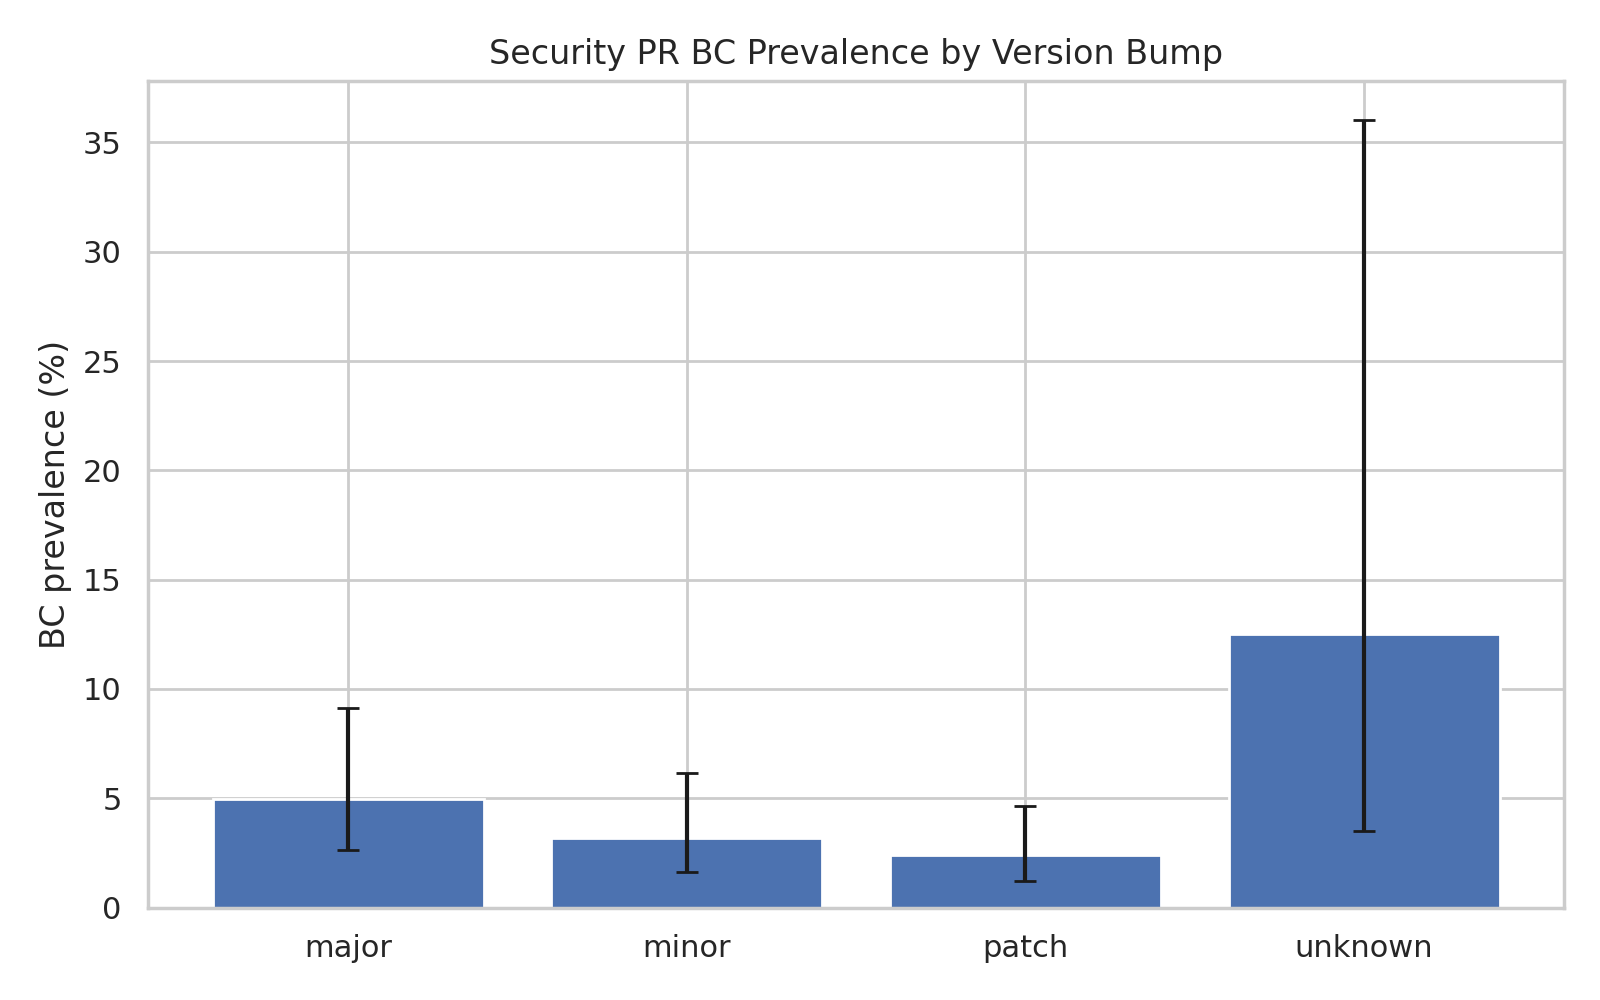
\includegraphics[width=\columnwidth]{../results/figures/rq1_prevalence_by_bump.png}
\caption{BC prevalence by version bump type, analyzed-only rows (corrected).}
\label{fig:bump}
\end{figure}

\subsection{RQ2: Predictive Model}
\label{sec:rq2}
We trained four classifiers on \texttt{analyzed\_ok} rows (380 PRs, 109 distinct repositories) using repository stars, version bump type, CVSS-derived features, ecosystem, CVE presence, and top CWE categories. We evaluate with repeated, repository-grouped cross-validation (\texttt{StratifiedGroupKFold}, 5 repeats $\times$ 5 folds = 25 evaluations per model) so that no repository appears in both the training and test partition of a fold, and report mean $\pm$ standard deviation AUC-ROC rather than a single train/test split. Table~\ref{tab:rq2} reports results, including a \texttt{DummyClassifier} (most-frequent-class) baseline to contextualize how much the real models add over chance-level performance given class balance.

\begin{table}[t]
\caption{RQ2 model performance (corrected, repeated grouped CV)}
\label{tab:rq2}
\centering
\begin{tabular}{lr}
\toprule
Model & Mean AUC-ROC $\pm$ std \\
\midrule
Dummy (most frequent) & $0.500 \pm 0.000$ \\
Logistic Regression & $0.849 \pm 0.082$ \\
\textbf{Random Forest} & $\mathbf{0.894 \pm 0.069}$ \\
Gradient Boosting & $0.879 \pm 0.067$ \\
Decision Tree & $0.794 \pm 0.106$ \\
\bottomrule
\end{tabular}
\end{table}

The best model, Random Forest, reaches mean AUC-ROC $0.894\pm0.069$ across 25 folds, well above the $0.500$ trivial baseline. The top features (fit on the full \texttt{analyzed\_ok} set) are repository stars (importance 0.381), ecosystem (0.188), CVSS score (0.116), version-bump magnitude (0.075), and ordinal CVSS severity (0.066); CWE categories contribute smaller, individually modest amounts. \texttt{has\_behavioral\_bc} is excluded from the feature set on principle -- it is derived from post-update test execution and is not a legitimate pre-outcome predictor, independent of whatever importance it might show. We also re-checked \texttt{has\_cve} after that removal: its importance is negligible (0.004, rank 15 of 16), a genuine finding rather than a leak, since CVE presence is a pre-outcome feature by construction (this dataset only contains CVE-linked security PRs, so \texttt{has\_cve} has little variance left to exploit).

For interpretability, we also fit logistic regressions via \texttt{statsmodels} to obtain coefficients with 95\% confidence intervals (sklearn's implementation does not expose these directly). The full-feature fit is singular, and even after excluding the quasi-separated \texttt{cwe\_CWE\_476} column a further exact collinearity remains among sparse one-hot predictors, so we report only the reduced full-rank refit. In that refit, ecosystem (Maven vs.\ PyPI) is a strong, significant predictor even controlling for CVSS and version bump ($\beta=-5.26$, 95\% CI $[-6.81,-3.70]$, $p=3.7\times10^{-11}$; PyPI predicts markedly lower BC odds), and version-bump magnitude remains significant ($\beta=0.68$, 95\% CI $[0.25,1.11]$, $p=0.002$); CVSS score and repository stars are not significant once ecosystem and bump magnitude are controlled for ($p=0.36$ and $p=0.36$ respectively), suggesting the Random Forest's use of \texttt{repo\_stars} captures nonlinear or interaction effects a linear model does not.

\begin{figure}[t]
\centering
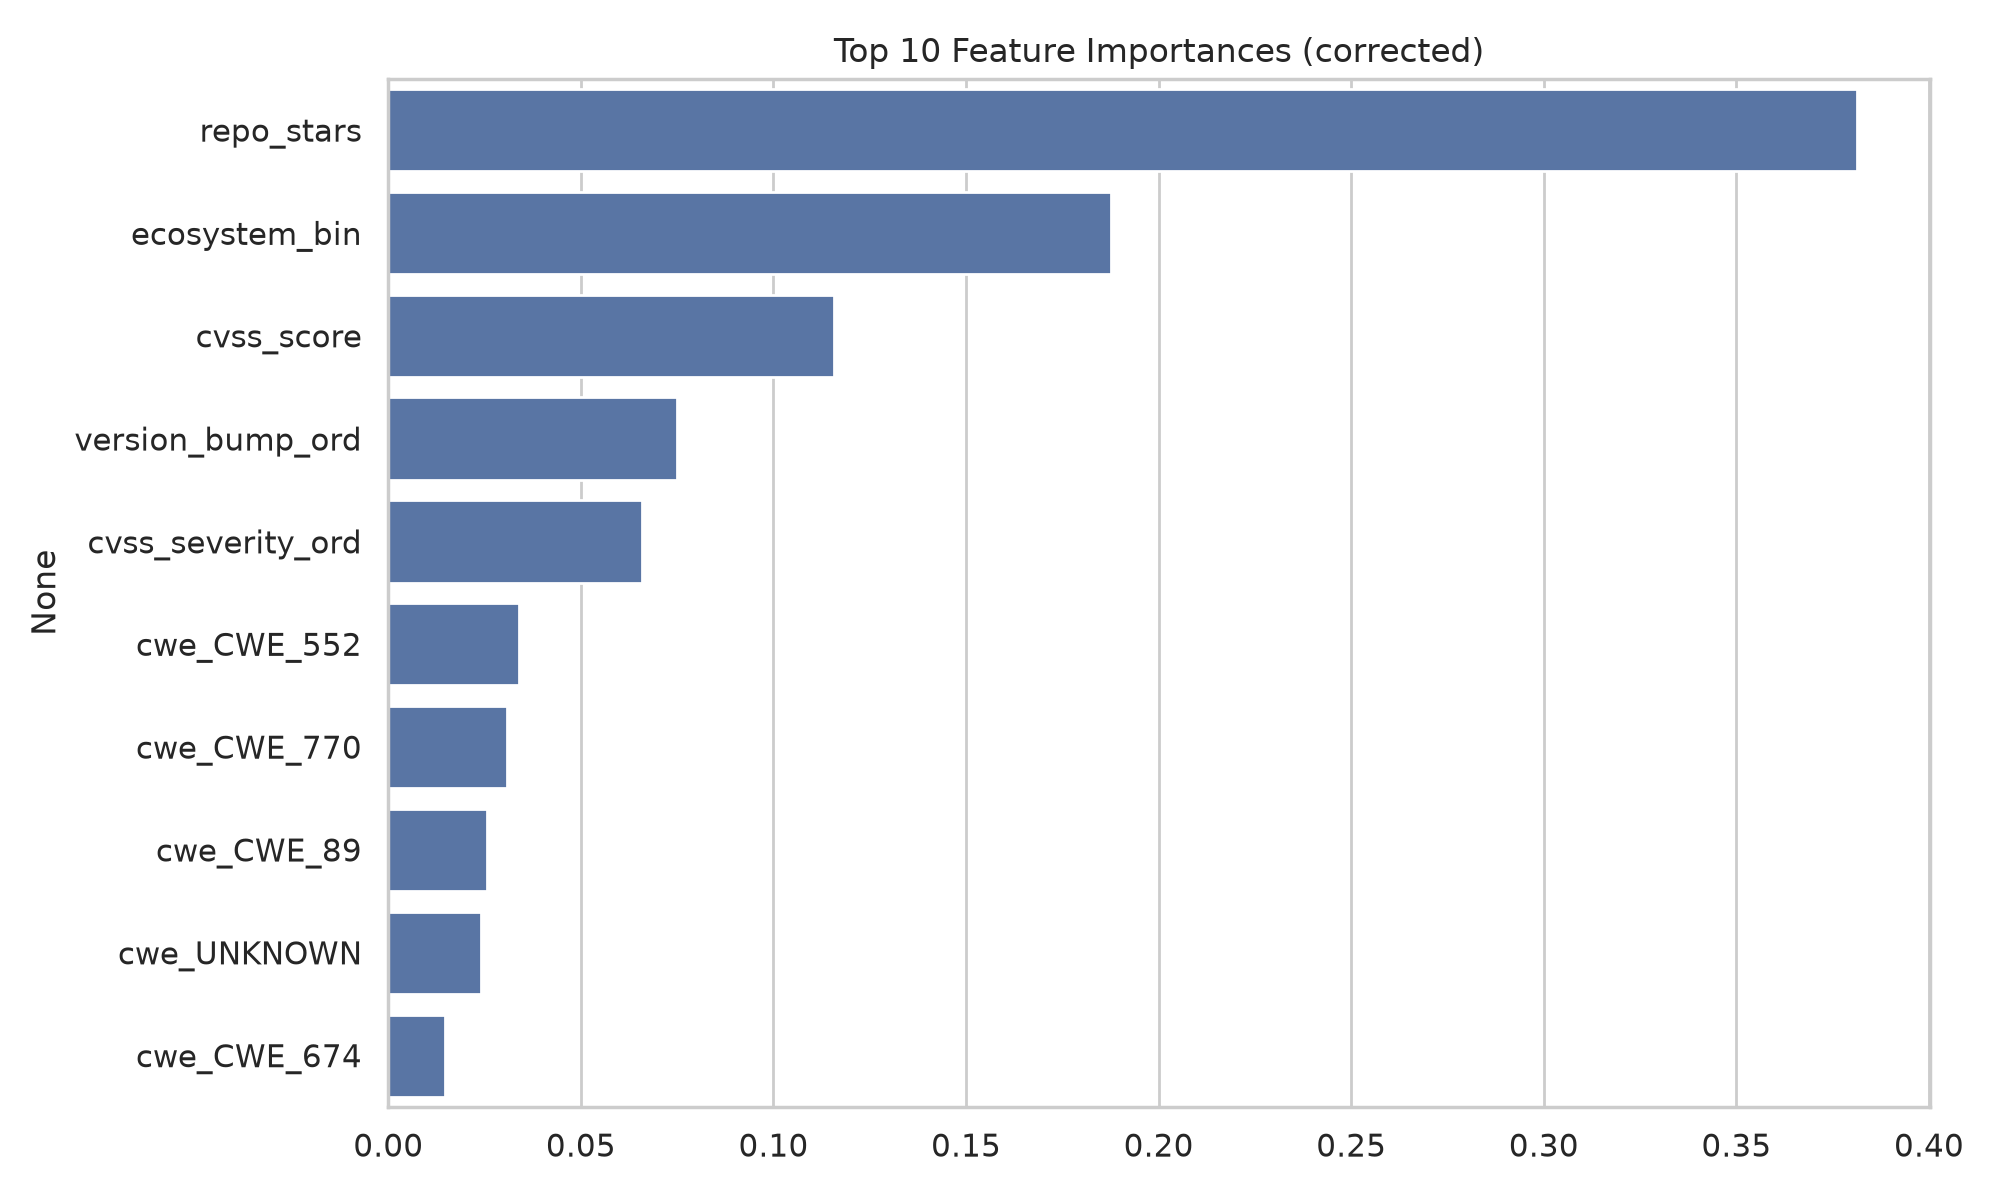
\includegraphics[width=\columnwidth]{../results/figures/rq2_feature_importance.png}
\caption{Feature importance for the best predictive model (corrected).}
\label{fig:importance}
\end{figure}

\subsection{RQ3: Team Response}
\label{sec:rq3}
Among the 160 BC-introducing PRs, 54 were merged anyway (33.8\%). Measuring follow-up remediation requires identifying, among PRs opened after the merge, which ones are actually fixing the BC rather than coincidentally containing a word like ``fix'' in an active repository. A naive keyword-only match (title/body contains ``fix'', ``revert'', ``repair'', ``downgrade'', or ``rollback'') finds 784 candidate PRs across the 160 BC PRs; requiring in addition that a candidate reference the original PR number, touch the same dependency manifest file, or mention the dependency by name leaves 248 (31.6\% of naive candidates survive; 68.4\% were unrelated). This relatedness filter changes the headline remediation numbers substantially: the naive median time-to-fix of 1.0 day (IQR 0.1--3.5) becomes \textbf{3.5 days (IQR 0.8--10.4)} under the strict filter, with 20.0\% fixed within seven days (vs.\ 28.1\% naive) and 25.6\% within 30 days (vs.\ 31.2\% naive); the reversion rate drops from 14.4\% (naive) to 8.8\% (strict). We report the strict numbers as the paper's cited remediation-speed figures going forward. CI failures in the post-merge window are measured independently of this keyword-relatedness issue and are unaffected. As in the uncorrected analysis, the logistic regression for fast remediation does not converge (singular design matrix) given the covariate structure; we do not report coefficients from it.

\section{Discussion}
The rectification (Section~\ref{sec:rectification}) was not a modest correction. Within every version-bump stratum, the rows it recovered show 6--9$\times$ higher BC rates than the original 201-row analyzed set (e.g., 69.3\% vs.\ 10.0\% for patch bumps). We manually verified a sample of the recovered dependency matches against real, well-documented major upgrades (e.g., H2 Database 1.4.190~$\to$~2.1.210, Jetty 9.4~$\to$~10.0, Guava 30~$\to$~32, Hibernate 5.2~$\to$~5.4) and found the matches and reported BC counts plausible in every case checked. The bug was not excluding a random subset of PRs; it disproportionately excluded older-style Dependabot PRs for legacy, heavyweight dependencies that had accumulated more API surface change by the time of the security bump -- exactly the PRs most likely to break something. Fixing it flips the paper's central comparison against the provider-side baseline from ``client-side risk is lower than metadata suggests'' to ``client-side risk, where we can measure it, is substantially higher.''

The broader message is not that security PRs are ``safe'' or ``unsafe'' in the abstract, but that measuring client-side compatibility risk requires verifying that measurement actually happened for a given PR before treating its absence of a positive signal as a negative result. A partially-run detector and a detector that ran and found nothing are different findings, and conflating them changed this paper's conclusion by an order of magnitude -- and the same discipline applied to RQ3's remediation-speed measurement (Section~\ref{sec:threats} and the strict-vs-naive comparison in RQ3) cut the apparent median fix time by more than a factor of three once unrelated PRs were filtered out. Both corrections point the same direction: a number computed over the wrong population, even with a correct formula, is not a smaller version of the truth.

\section{Threats to Validity}
\label{sec:threats}
This study has several limitations, some inherited from the original design and some specific to the correction described in Section~\ref{sec:rectification}.

\emph{Coverage and representativeness.} Even after correction, BC detection genuinely executed for only 48.5\% of the cohort (380/783), and the analyzed subset is demonstrably \emph{not} a random sample of it: analyzed rows skew toward lower-star repositories (median 9{,}234 vs.\ 16{,}684 stars, Mann-Whitney $p=3.65\times10^{-21}$), toward PyPI rather than Maven rows (36.6\% vs.\ 22.3\% PyPI among unanalyzed, $\chi^2$ $p=1.7\times10^{-5}$), and toward unmerged PRs (44.2\% merged among analyzed vs.\ 61.0\% among unanalyzed, $\chi^2$ $p=3.4\times10^{-6}$); version-bump-type mix still does not differ significantly ($p=0.777$), so coverage is not biased by bump magnitude itself. We quantify the consequence directly in Section~\ref{sec:robustness} rather than leaving it as an unquantified caveat: worst-case bounds of [20.4\%, 71.9\%] and a model-based imputed estimate of 38.0\% both bracket the cited 42.1\%, but do not pin it down precisely -- further ecosystem-retagging or broader artifact-resolution work could move the estimate within that range.

\emph{Residual known issues, not fixed in this pass.} Ecosystem (Maven vs.\ PyPI) is assigned from repository-root file presence at collection time, not from what a given PR actually modifies; in polyglot repositories this misclassifies some GitHub Actions and npm/pip Dependabot bumps as Maven rows, which are correctly left unanalyzable (no Maven coordinate exists to resolve) but add noise to the Maven/PyPI comparison we could not fully separate from genuine ecosystem-level differences. Behavioral BC is not reported, not merely conservative: two structural bugs in the test harness are fixed and verified (Section~\ref{sec:rectification}), but the resulting pass/fail signal is still dominated by environment confounds (missing test-only dependencies, registry rate-limiting) rather than genuine pre/post-update outcomes, so we report it as unmeasured future work rather than publish an unreliable percentage.

\emph{Java analysis is stronger than Python.} Maven projects use Roseau, a source/bytecode-level compatibility checker; PyPI projects use a lighter public-API signature comparison. This asymmetry predates this correction and remains unresolved.

\emph{Vulnerability metadata quality.} Recent work reports that a large fraction of vulnerability-database entries carry incorrect package coordinates or affected-version ranges~\cite{nvdquality2026}. Our analysis inherits CVE metadata from the NVD, but the artifacts it actually diffs are the concrete \texttt{old\_version}$\to$\texttt{new\_version} pair named in each Dependabot PR, not an NVD version range. As a direct check, we drew a random sample of 100 CVE-linked Maven PRs from the analyzed set and verified each claimed-vulnerable (\texttt{old\_version}) and fixed (\texttt{new\_version}) coordinate against Maven Central: all 100 of both resolved to real published artifacts (0\% mismatch; \texttt{data/nvd\_metadata\_validation.csv}). This rules out the ``phantom version'' failure mode for the measured subset -- every BC we report is computed between two artifacts that demonstrably exist -- but it does not verify that each CVE's severity or affected-range semantics are themselves correct, which we do not independently audit.

\emph{RQ3} relies on GitHub activity heuristics -- follow-up PR titles, branch activity, commit-status checks -- which are imperfect proxies for maintenance response; Section~\ref{sec:rq3} shows how much naive keyword matching alone can overstate remediation speed, and a relatedness filter was applied for exactly that reason, but the filter itself (PR-number reference, manifest-file overlap, or dependency-name mention) is still a heuristic, not ground truth.

Finally, the final cohort (783 unique PRs) is smaller than the 2{,}000-PR target originally sought by the collection process, which limits external validity beyond the repositories and time window studied.

\section{Conclusion}
SecBreak provides an empirical, client-side view of breaking changes in automated security updates, and a transparent account of a pipeline bug that inverted its own headline finding. Across the 380 Dependabot security PRs (of 783 in the cohort) where breaking-change detection genuinely executed, 42.1\% introduce a syntactic BC -- significantly \emph{higher} than the 13.2\% provider-side metadata baseline, not lower. Maven PRs carry nearly all of the observed risk (65.6\% vs.\ 1.4\% for PyPI); even patch-level updates introduce a BC 37.3\% of the time. Our main contribution is this prevalence estimate for a narrow but operationally important population: automated security-fix PRs under real client projects. A repository-grouped, repeatedly cross-validated model reaches AUC-ROC $0.894\pm0.069$ without target leakage, but we treat prediction as supporting triage evidence rather than the paper's novelty claim. Teams merge a third of BC-inducing security PRs anyway and, when they remediate in a way that plausibly relates to the dependency bump, typically do so within about a week (median 3.5 days). We do not report a behavioral BC number: two structural bugs in the test-based harness are fixed and verified, but a diagnostic run showed the resulting signal is still dominated by environment confounds, and we would rather report that honestly as future work than publish an unreliable percentage. The practical implication is unchanged in direction but sharper in magnitude: security automation should surface compatibility-risk evidence alongside vulnerability severity, and any pipeline that measures that risk should make its own completeness -- not just its output -- part of the reported result.

\section{Replication Package}
The repository contains, for both the original (buggy) and corrected pipeline runs:
\begin{itemize}
\item corrected dataset: \texttt{data/analysis\_dataset\_corrected.csv} (original: \texttt{data/analysis\_dataset.csv})
\item cohort manifest: \texttt{results/cohort/frozen\_cohort.csv}
\item cohort flow: \texttt{results/cohort/cohort\_flow.json}
\item corrected validation package: \texttt{results/validation/bc\_validation\_sample\_corrected.csv} (original: \texttt{results/validation/bc\_validation\_sample.csv})
\item corrected RQ1/RQ2/RQ3 tables: \texttt{results/rq\{1,2,3\}\_tables\_corrected.csv} (originals suffixed \texttt{\_ORIGINAL\_BUGGY}; strict RQ3 relatedness-filtered table: \texttt{results/rq3\_tables\_strict.csv})
\item model outputs: \texttt{results/rq2\_model\_results\_corrected.csv}, logistic-regression coefficients with CIs: \texttt{results/rq2\_logit\_coefficients\_converged.csv}
\item robustness bounds (Section~\ref{sec:robustness}): \texttt{results/rq1\_bounds.json}
\item selection-bias quantification: \texttt{results/selection\_bias\_table.csv}
\item NVD affected-version metadata validation: \texttt{data/nvd\_metadata\_validation.csv} (script: \texttt{nvd\_metadata\_validation.py})
\item Maven-only vs.\ dual-ecosystem comparison: \texttt{results/MAVEN\_ONLY\_COMPARISON.md} and \texttt{results/*\_mavenonly.csv}
\item validation review aids (PR-diff/changelog links, formatted detector output): \texttt{results/validation/review\_context.jsonl}
\item full rectification report and decision trail: \texttt{results/RECTIFICATION\_REPORT.md}; paper-strengthening report: \texttt{results/STRENGTHENING\_REPORT.md}
\end{itemize}

\begin{thebibliography}{20}
\bibitem{raemaekers2021}
S.~Raemaekers, A.~van Deursen, and J.~Visser, ``Do Security Updates Break Compatibility? An Empirical Study of Versioning in Security Releases,'' \emph{IEEE Transactions on Software Engineering}, 2021.

\bibitem{dietrich2014semver}
J.~Dietrich, K.~Jezek, and P.~Brada, ``Broken Promises: An Empirical Study into Evolution Problems in Java Programs Caused by Library Upgrades,'' in \emph{Proc.\ Software Evolution Week -- IEEE Conf.\ on Software Maintenance, Reengineering, and Reverse Engineering (CSMR-WCRE)}, 2014, pp.\ 64--73.

\bibitem{raemaekers2017semver}
S.~Raemaekers, A.~van Deursen, and J.~Visser, ``Semantic Versioning and Impact of Breaking Changes in the Maven Repository,'' \emph{Journal of Systems and Software}, vol.\ 129, pp.\ 140--158, 2017.

\bibitem{ochoa2022maven}
L.~Ochoa, T.~Degueule, J.-R.~Falleri, and J.~Vinju, ``Breaking Bad? Semantic Versioning and Impact of Breaking Changes in Maven Central,'' \emph{Empirical Software Engineering}, vol.\ 27, 2022.

\bibitem{jayasuriya2024emse}
D.~Jayasuriya, S.~Ou, S.~Hegde, V.~Terragni, J.~Dietrich, and K.~Blincoe, ``An Extended Study of Syntactic Breaking Changes in the Wild,'' \emph{Empirical Software Engineering}, vol.\ 29, 2024.

\bibitem{kula2018emse}
R.~G.~Kula, D.~M.~German, A.~Ouni, T.~Ishio, and K.~Inoue, ``Do Developers Update Their Library Dependencies? An Empirical Study on the Impact of Security Advisories on Library Migration,'' \emph{Empirical Software Engineering}, vol.\ 23, no.\ 1, pp.\ 384--417, 2018.

\bibitem{hejderup2021}
J.~Hejderup and G.~Gousios, ``Can We Trust Tests To Automate Dependency Updates? A Case Study of Java Projects,'' \emph{Journal of Systems and Software}, vol.\ 183, p.\ 111097, 2021.

\bibitem{rombaut2024}
B.~Rombaut, F.~R.~Cogo, and A.~E.~Hassan, ``Leveraging the Crowd for Dependency Management: An Empirical Study on the Dependabot Compatibility Score,'' \emph{arXiv preprint arXiv:2403.09012}, 2024.

\bibitem{venturini2023}
D.~Venturini, F.~R.~Cogo, I.~Polato, M.~A.~Gerosa, and I.~S.~Wiese, ``I Depended on You and You Broke Me: An Empirical Study of Manifesting Breaking Changes in Client Packages,'' \emph{ACM Transactions on Software Engineering and Methodology}, vol.\ 32, no.\ 4, 2023.

\bibitem{breakguard2026}
R.~Raj, B.~Baudry, and D.~E.~Costa, ``BreakGuard: Towards Detecting Dependency Breaking Changes with LLM-Generated Tests,'' \emph{arXiv preprint arXiv:2608.20167}, 2026.

\bibitem{nvdquality2026}
Y.~Nong, Y.~Du, T.~Xu, and H.~Cai, ``The Data Problem in Software Vulnerability Analysis: Artifacts, Quality, and Consumption,'' \emph{arXiv preprint arXiv:2609.01503}, 2026.

\bibitem{alfadel2021}
M.~Alfadel, D.~Costa, E.~Shihab, and M.~Mkhallalati, ``On the Use of Dependabot Security Pull Requests,'' in \emph{Proc.\ IEEE/ACM 18th Working Conf.\ on Mining Software Repositories (MSR)}, 2021, pp.\ 254--265.

\bibitem{rebatchi2024}
H.~Rebatchi, T.~F.~Bissyand{\'e}, and N.~Moha, ``Dependabot and Security Pull Requests: Large Empirical Study,'' \emph{Empirical Software Engineering}, vol.\ 29, 2024.

\bibitem{mohayeji2023}
H.~Mohayeji, A.~Agaronian, E.~Constantinou, N.~Zannone, and A.~Serebrenik, ``Investigating the Resolution of Vulnerable Dependencies with Dependabot Security Updates,'' in \emph{Proc.\ IEEE/ACM 20th Working Conf.\ on Mining Software Repositories (MSR)}, 2023.

\bibitem{mohayeji2025}
H.~Mohayeji, A.~Agaronian, E.~Constantinou, N.~Zannone, and A.~Serebrenik, ``Securing Dependencies: A Comprehensive Study of Dependabot's Impact on Vulnerability Mitigation,'' \emph{Empirical Software Engineering}, vol.\ 30, 2025.

\bibitem{fruntke2025}
L.~Fruntke and J.~Krinke, ``Automatically Fixing Dependency Breaking Changes,'' \emph{Proceedings of the ACM on Software Engineering}, vol.\ 2, no.\ FSE, 2025.

\bibitem{byam2025}
F.~Reyes, M.~Mahmoud, F.~Bono, S.~Nadi, B.~Baudry, and M.~Monperrus, ``Byam: Fixing Breaking Dependency Updates with Large Language Models,'' \emph{arXiv preprint arXiv:2505.07522}, 2025.
\end{thebibliography}

\end{document}
